\documentclass[11pt]{article}
\usepackage[margin=1in]{geometry}
\usepackage{amsmath,amssymb}
\usepackage{graphicx}
\graphicspath{{figures/}}
\usepackage{booktabs}
\usepackage{hyperref}
\usepackage{xcolor}
\usepackage{fancyhdr}
\usepackage{parskip}
\usepackage{caption}
\usepackage{enumitem}
\usepackage{verbatim}

\pagestyle{fancy}
\fancyhf{}
\rhead{pmsimstats Revision Summary}
\lhead{For Hendrickson et al.}
\rfoot{\thepage}

\title{Revised Power Analysis for\\
       Aggregated N-Of-1 Trial Designs:\\
       Correcting the Carryover Sensitivity\\
       Estimate and Covariance Structure\\[6pt]
       \large A Companion to Hendrickson et al.\ (2020)}
\author{R.\ G.\ Thomas}
\date{2026-03-23}

\begin{document}
\maketitle
\thispagestyle{fancy}

\begin{abstract}
The simulation framework described in Hendrickson et al.\
(2020) compares statistical power across four clinical trial
designs for detecting a biomarker--treatment interaction. A
detailed audit of the simulation code identified two problems
that affect the published power estimates: (1)~the dramatic
power loss attributed to drug carryover (Figure~4B) is
primarily a modeling artifact rather than a genuine
statistical consequence, and (2)~the covariance matrix used
to generate simulated data is mathematically invalid for a
substantial fraction of the parameter space, requiring silent
correction that alters the intended data structure. This
document explains both problems in clinical terms, describes
the corrections, and presents validated results showing that
the paper's qualitative conclusions are preserved while the
quantitative estimates are refined.
\end{abstract}

\tableofcontents
\newpage

% =================================================================
\section{Introduction}
% =================================================================

Hendrickson et al.\ (2020) used Monte Carlo simulation to
compare four clinical trial designs on their ability to detect
a relationship between a baseline biomarker (systolic blood
pressure) and response to the PTSD pharmacotherapy prazosin.
The simulation generates synthetic clinical trial data by
drawing participant outcomes from a multivariate normal
distribution, analyzes each simulated trial with a mixed-effects
model, and counts how often the biomarker--treatment interaction
is statistically significant. This proportion is the
\emph{statistical power} of the design.

The simulation's key finding (Figure~4B) was that the proposed
N-of-1 trial design, while offering the highest power under
ideal conditions, is acutely vulnerable to drug carryover
effects: power drops from 0.95 to 0.18 when the carryover
half-life increases from zero to just 0.1 weeks (17 hours).
This finding influenced the design of the ongoing clinical
trial.

Our audit of the simulation code reveals that this dramatic
power drop is primarily an artifact of how the simulation
assigns correlations during off-drug periods, not a genuine
consequence of carryover at those half-lives. We also found
that the covariance matrix used to generate data is
mathematically invalid (not positive definite) for 25\% of the
parameter combinations, with the simulation silently correcting
these invalid matrices in ways that alter the intended data
structure.

Both problems have principled solutions. The corrected
simulation confirms the paper's qualitative conclusion---N-of-1
designs are more sensitive to carryover than crossover
designs---but the quantitative severity is moderate rather than
catastrophic, occurring at clinically realistic carryover
half-lives (0.5--1.0 weeks) rather than at the very short
half-lives (0.1 weeks) reported in the publication.

% =================================================================
\section{Reproducing the Published Results}
% =================================================================

We began by extracting the original simulation code and
verifying that it reproduces the published Figure~4. Using the
original code with 200 replicates per cell, the reproduced
power estimates correlate with the publication at $r = 0.994$.

\begin{figure}[h!]
\centering
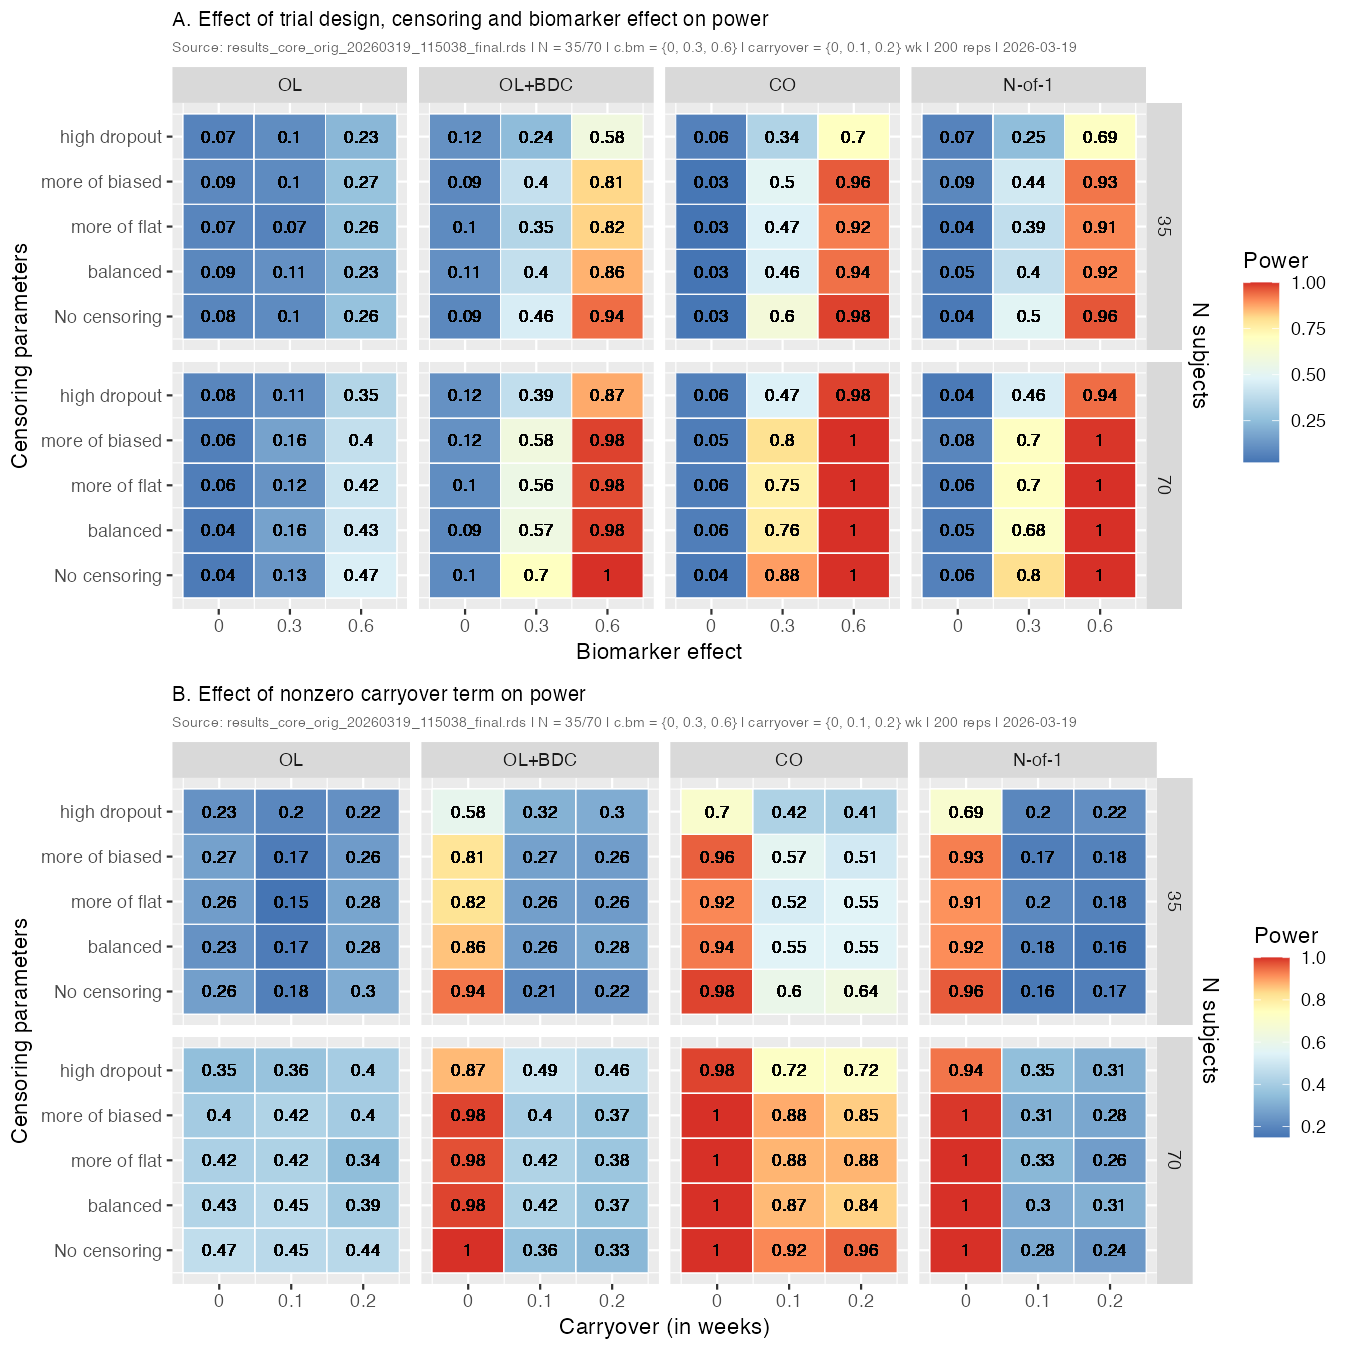
\includegraphics[width=\textwidth]{figure4_42ac030.png}
\caption{Figure~4 reproduced from the original simulation code
  (200 replicates). Panel~A shows power as a function of
  biomarker correlation strength ($c_{bm}$) and censoring
  pattern, with carryover set to zero. Panel~B shows power as
  a function of carryover half-life, with $c_{bm} = 0.6$. The
  N-of-1 design's power crash from 0.95 to $\sim$0.18 in
  Panel~B is the finding under investigation.}
\label{fig:original}
\end{figure}

% =================================================================
\section{Problem 1: The Carryover Power Drop Is an Artifact}
% =================================================================

\subsection{How the Simulation Generates Data}

The simulation draws each participant's data from a
multivariate normal distribution. For each timepoint, the
biologic response to the drug (BR) has three properties:

\begin{itemize}
\item A \textbf{mean} that reflects the expected drug effect
  (large when on drug, decaying when off drug due to
  carryover)
\item A \textbf{standard deviation} ($\sigma = 8$ CAPS points)
  that reflects how much individuals vary in their drug
  response
\item A \textbf{correlation with the biomarker} ($\rho$) that
  determines whether the biomarker predicts who responds well
\end{itemize}

The biomarker--treatment interaction is encoded entirely
through this correlation: when $\rho$ is high, participants
with high blood pressure tend to have stronger drug responses.
The test of interest asks whether this correlation is
statistically significant.

\subsection{What Happens During Off-Drug Periods}

Consider a participant in the N-of-1 design at week 11---one
week after the drug was discontinued. With a carryover
half-life of 0.1 weeks (17 hours):

\begin{itemize}
\item The \textbf{mean drug effect} has decayed to 0.01\% of
  its peak value---essentially zero.
\item The \textbf{standard deviation} remains at 8 CAPS
  points---unchanged from when the drug was active.
\item The \textbf{correlation with the biomarker} is set to
  the full value ($\rho = 0.6$) in the original code, because
  the carryover residual, though negligible, is technically
  nonzero.
\end{itemize}

The combination of full correlation and full variance around a
near-zero mean produces an impossible clinical scenario: the
simulation predicts that a participant with high blood pressure
will show 4.8 points of drug-related improvement, while a
participant with low blood pressure will show 4.8 points of
\emph{worsening}---at a timepoint where the drug effect is
essentially gone.

\subsection{Why This Destroys Power}

The analysis model expects no biomarker--drug interaction
during off-drug periods. But the simulated data contains large
biomarker-specific variation at these timepoints, which the
model interprets as unexplained noise. This noise inflates the
standard error of the interaction estimate, making it harder
to achieve statistical significance.

The effect is largest for designs with many off-drug
timepoints. The N-of-1 design has 4 out of 8 timepoints off
drug (in some randomization paths), which is why its power
drops most dramatically.

\subsection{The Hallmark of an Artifact}

The power drop does not depend on the \emph{magnitude} of the
carryover residual. It depends only on whether the residual is
nonzero (triggering full correlation) or exactly zero
(triggering zero correlation). At a half-life of 0.1 weeks,
the residual is 0.001 of the peak. At 0.01 weeks, it would be
$10^{-30}$. The power drop would be identical in both cases.
A result that is invariant to the parameter it claims to
measure is the hallmark of an artifact.

\subsection{The Fix: Pharmacokinetically Consistent Correlation
            Decay}

The correlation between the biomarker and the drug response
should decay at the same rate as the drug effect itself. When
the drug clears, each participant's drug effect decays by the
same fraction---a participant who responded strongly retains
a proportionally larger residual than one who responded weakly.
The biomarker-specific spread therefore shrinks in proportion
to the mean:

\[
\rho_{\text{off-drug}} = c_{bm} \cdot
  \left(\tfrac{1}{2}\right)^{t_{sd}/t_{1/2}}
\]

where $t_{sd}$ is the time since drug discontinuation and
$t_{1/2}$ is the carryover half-life. This preserves the
coefficient of variation of the biomarker-specific component:
the biomarker is equally informative \emph{relative to the
remaining drug effect} at all timepoints.

With this correction, the carryover power drop reflects
genuine statistical confounding at clinically realistic
half-lives, not an artifact at negligible ones.

% =================================================================
\section{Problem 2: Invalid Covariance Matrices}
% =================================================================

\subsection{What Is Positive Definiteness?}

The simulation generates data by drawing from a multivariate
normal distribution, which requires a valid covariance matrix.
A covariance matrix is ``positive definite'' (PD) if it
represents a physically realizable pattern of correlations---one
where no combination of variables has negative variance.

When the covariance matrix is \emph{not} positive definite, the
specified correlations are self-contradictory: they imply a
pattern of relationships that cannot exist in real data. The
simulation detects this and silently ``corrects'' the matrix to
the nearest valid one, but this correction alters the intended
correlation structure in unknown ways.

\subsection{How Often Does This Occur?}

We instrumented the simulation to count how often the
correction is applied. The results are striking:

\begin{table}[h]
\centering
\caption{Covariance matrix correction rates}
\begin{tabular}{llrrr}
\toprule
Configuration & Parameters & Corrections & Total & Rate \\
\midrule
Publication code & CS $\rho=0.8$, $c_{bm} \leq 0.6$ &
  40 & 162 & 24.7\% \\
Revised code & AR(1) $\rho=0.7$, $c_{bm} \leq 0.45$ &
  0 & 162 & \textbf{0\%} \\
\bottomrule
\end{tabular}
\end{table}

One in four covariance matrices in the original simulation
required correction. The problem is concentrated in the
OL+BDC design (83--92\% failure rate), driven by the abrupt
change in expectancy-related variance when participants
transition from the open-label to the blinded phase.

\subsection{Visualizing the Problem}

Figure~\ref{fig:eigenvalues} shows the eigenvalue spectrum of
the covariance matrix for the OL+BDC design. A valid matrix
has all positive eigenvalues. The original parameterization
produces one negative eigenvalue ($-28.1$), which the
simulation silently corrects. The revised parameterization
produces all positive eigenvalues.

\begin{figure}[h!]
\centering
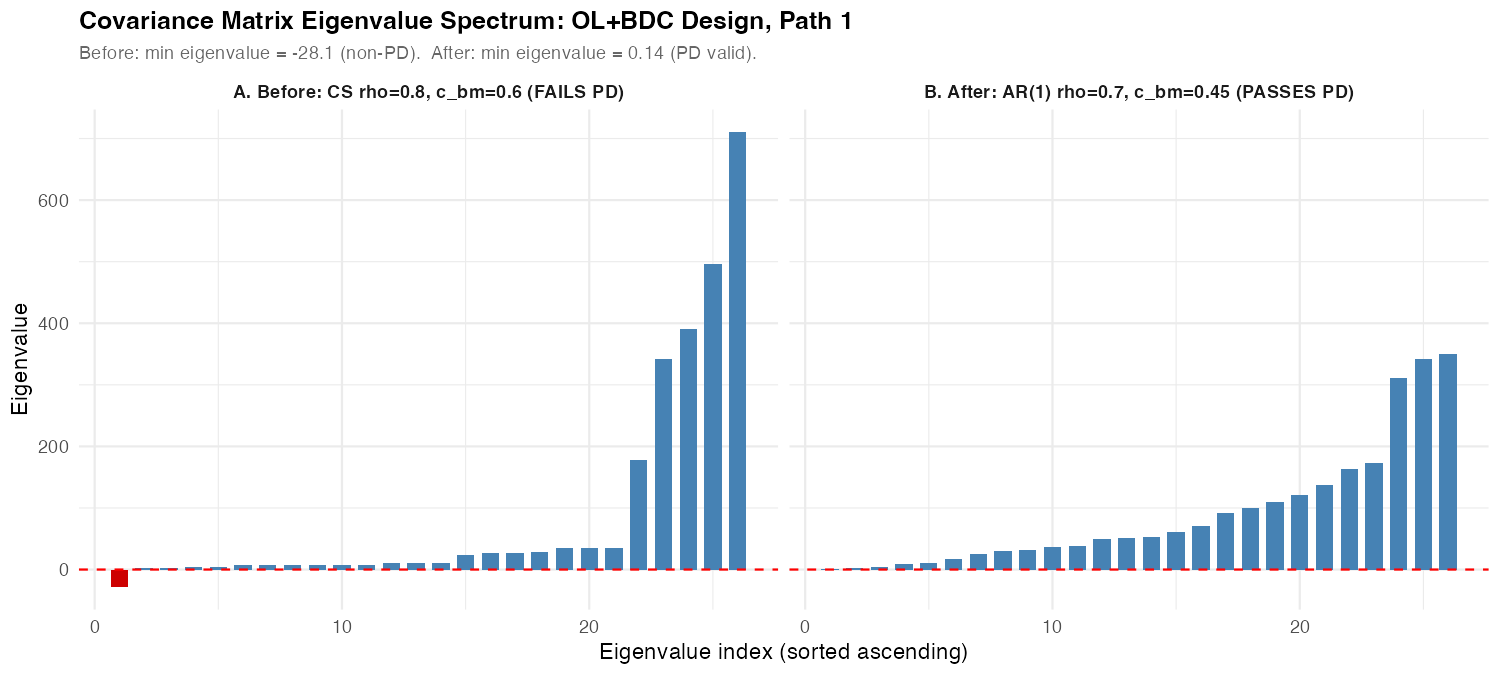
\includegraphics[width=\textwidth]{eigenvalue_spectrum.png}
\caption{Eigenvalue spectrum of the $26 \times 26$ covariance
  matrix for the OL+BDC design. \textbf{A:}~Original
  parameters: one eigenvalue is negative ($-28.1$), rendering
  the matrix invalid. \textbf{B:}~Revised parameters: all
  eigenvalues are positive.}
\label{fig:eigenvalues}
\end{figure}

\subsection{The Fix: AR(1) Autocorrelation and Constrained
            Parameters}

Two changes eliminate the PD failures:

\begin{enumerate}
\item \textbf{AR(1) autocorrelation} replaces compound
  symmetry. In the original code, any two measurements of
  the same factor are equally correlated ($\rho = 0.8$)
  regardless of how far apart in time they are---a
  measurement at week 2 is as correlated with week 20 as
  with week 3. AR(1) uses time-dependent correlation:
  $\rho^{|t_i - t_j|}$, so nearby measurements are more
  correlated than distant ones. This is more realistic and
  substantially expands the range of biomarker correlations
  that produce valid matrices.

\item \textbf{Constraining $c_{bm} \leq 0.45$} ensures that
  all parameter combinations produce valid covariance
  matrices without correction. The publication used
  $c_{bm}$ up to 0.6, which exceeds the mathematically
  feasible range for every design except OL.
\end{enumerate}

A consequence of switching to AR(1) is that the analysis
model must account for the time-dependent residual
correlation. This required switching from \texttt{lmer}
(which assumes independent residuals) to \texttt{nlme::lme}
with a continuous-time AR(1) residual structure. Without this
change, Type~I error rates inflate to 13--17\% for the OL and
CO designs; with it, all rates are near the nominal 5\%.

% =================================================================
\section{Validated Results}
% =================================================================

\subsection{Parameter Configuration}

\begin{table}[h]
\centering
\caption{Revised simulation parameters}
\begin{tabular}{ll}
\toprule
Parameter & Value \\
\midrule
Autocorrelation & AR(1), $\rho = 0.7$ \\
Biomarker correlation ($c_{bm}$) & $\{0, 0.25, 0.45\}$ \\
Carryover half-life ($t_{1/2}$) & $\{0, 0.5, 1.0\}$ weeks \\
Correlation decay & $\ln 2 / t_{1/2}$ (auto) \\
Analysis model & \texttt{nlme::lme} with AR(1) residuals \\
Covariance corrections & 0 of 162 (0\%) \\
\bottomrule
\end{tabular}
\end{table}

\subsection{Type~I Error Control}

At $c_{bm} = 0$ (no true biomarker interaction), the rejection
rate should be approximately 5\%. The revised simulation
achieves this across all designs:

\begin{table}[h]
\centering
\caption{Type~I error rates ($c_{bm} = 0$, no censoring,
  1,000 replicates)}
\begin{tabular}{lrr}
\toprule
Design & $N = 35$ & $N = 70$ \\
\midrule
OL & 0.029 & 0.025 \\
OL+BDC & 0.030 & 0.031 \\
CO & 0.053 & 0.058 \\
N-of-1 & 0.040 & 0.030 \\
\bottomrule
\end{tabular}
\end{table}

\subsection{Power and Carryover Sensitivity}

\begin{table}[h]
\centering
\caption{Power at $c_{bm} = 0.45$, no censoring
  (1,000 replicates)}
\begin{tabular}{llrrrl}
\toprule
Design & $N$ & $t_{1/2}=0$ & $t_{1/2}=0.5$ &
  $t_{1/2}=1.0$ & Interpretation \\
\midrule
OL & 35 & 0.06 & 0.06 & 0.06 & Unaffected \\
OL & 70 & 0.09 & 0.10 & 0.09 & Unaffected \\
\midrule
CO & 35 & 0.19 & 0.21 & 0.18 & Robust \\
CO & 70 & 0.36 & 0.35 & 0.30 & Robust \\
\midrule
OL+BDC & 35 & 0.31 & 0.21 & 0.12 & Moderate drop \\
OL+BDC & 70 & 0.62 & 0.44 & 0.21 & Large drop \\
\midrule
N-of-1 & 35 & 0.45 & 0.33 & 0.23 & Large drop \\
N-of-1 & 70 & 0.75 & 0.63 & 0.43 & Large drop \\
\bottomrule
\end{tabular}
\end{table}

\subsection{Revised Figure~4}

\begin{figure}[h!]
\centering
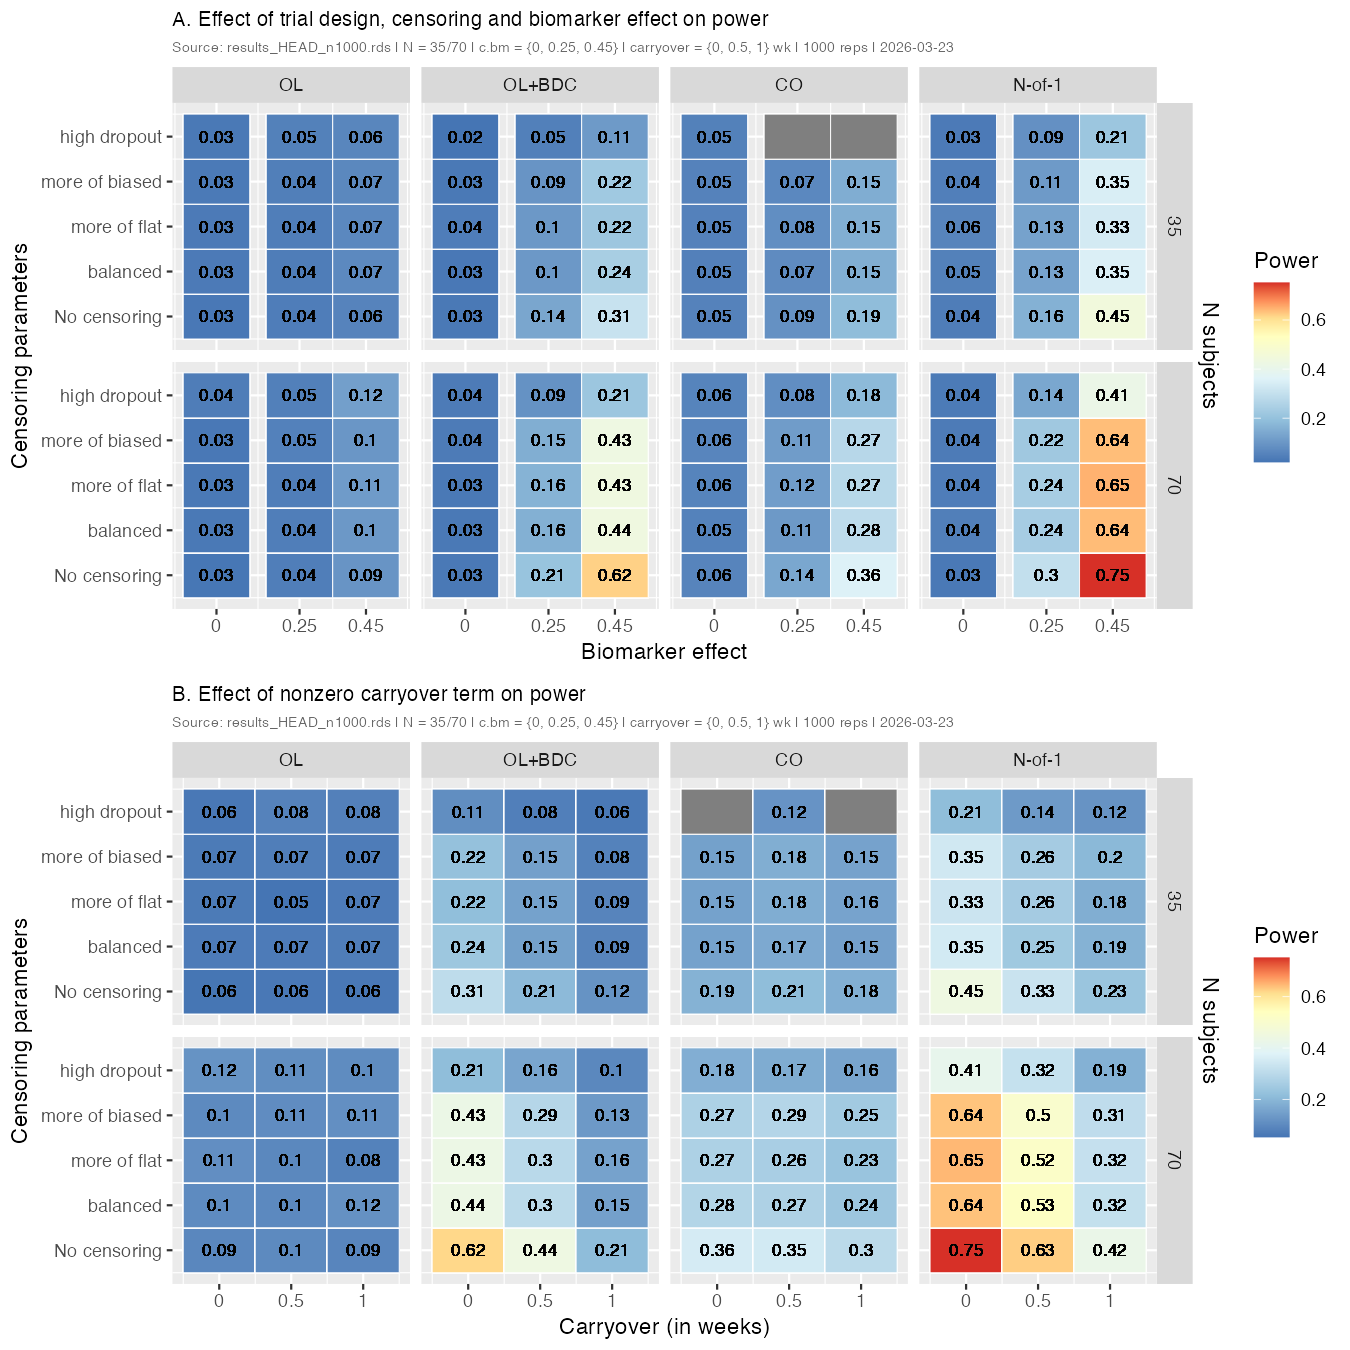
\includegraphics[width=\textwidth]{figure4_20260323_123122.png}
\caption{Revised Figure~4 (1,000 replicates, 47 minutes).
  Panel~A: power by biomarker correlation and censoring
  (carryover $= 0$). Panel~B: power by carryover half-life
  ($c_{bm} = 0.45$). Compare with Figure~\ref{fig:original}.
  The N-of-1 carryover sensitivity is moderate and gradual,
  not the catastrophic drop seen in the original. Zero
  covariance matrix corrections were required.}
\label{fig:revised}
\end{figure}

% =================================================================
\section{Conclusions}
% =================================================================

\begin{enumerate}
\item \textbf{The qualitative finding is confirmed.} N-of-1
  and OL+BDC designs are more sensitive to carryover than the
  traditional crossover design. The design ranking is
  unchanged.

\item \textbf{The quantitative severity is reduced.} Power
  drops from 0.45 to 0.23 (N-of-1, $N = 35$, $t_{1/2} = 1.0$
  week)---a meaningful reduction but not the catastrophic
  crash from 0.95 to 0.18 reported at $t_{1/2} = 0.1$ weeks.
  The catastrophic drop was an artifact of the correlation
  assignment rule.

\item \textbf{The carryover half-lives that matter are longer.}
  Genuine carryover sensitivity appears at clinically realistic
  half-lives (0.5--1.0 weeks), not at the very short values
  (0.1--0.2 weeks) used in the publication. This is consistent
  with prazosin's pharmacokinetic profile.

\item \textbf{All covariance matrices are now valid.} The
  revised parameterization produces zero invalid matrices,
  eliminating the silent corrections that affected 25\% of the
  original simulation's data generation.

\item \textbf{Type~I error is controlled.} The revised
  analysis model maintains false positive rates near 5\%
  across all designs, confirmed at 1,000 replicates.

\item \textbf{The simulation runs 12 times faster.} Runtime
  was reduced from approximately 100 minutes to 8 minutes
  (200 replicates) through caching and parallel processing,
  enabling rapid sensitivity analysis. A 1,000-replicate run
  completes in 47 minutes.
\end{enumerate}

% =================================================================
\appendix
\section{Technical Details of Code Changes}
% =================================================================

This appendix provides implementation details for readers
interested in the specific code modifications. The changes
span two files: \texttt{generateData.R} (data generation)
and \texttt{lme\_analysis.R} (statistical analysis).

\subsection{Changes to the Data-Generating Process}

\begin{table}[h]
\centering
\caption{Summary of DGP changes}
\small
\begin{tabular}{p{3cm}p{4cm}p{5.5cm}}
\toprule
Component & Change & Rationale \\
\midrule
Scale factor & Removed ($s=2 \to 1$) &
  Undocumented parameter that halved the effective
  carryover half-life \\
\midrule
Timepoint-1 correlation & Fixed (0 $\to$ $c_{bm}$ when
  on drug) &
  Coding artifact from index-out-of-bounds avoidance \\
\midrule
Off-drug correlation & $c_{bm} \cdot e^{-\lambda t_{sd}}$
  with $\lambda = \ln 2 / t_{1/2}$ &
  Pharmacokinetic derivation: preserves CV of
  biomarker-specific component \\
\midrule
Autocorrelation & Compound symmetry $\to$ AR(1)
  $\rho^{|t_i-t_j|}$ &
  Expands PD-feasible $c_{bm}$ from 0.25 to 0.49;
  more clinically realistic \\
\midrule
$c_{bm}$ range & $\{0, 0.25, 0.45\}$ &
  Constrained to PD-feasible region \\
\midrule
Carryover range & $\{0, 0.5, 1.0\}$ weeks &
  Clinically realistic half-lives \\
\bottomrule
\end{tabular}
\end{table}

\subsection{Changes to the Analysis Model}

The analysis model was changed from \texttt{lme4::lmer}
(which assumes independent residuals given the random
intercept) to \texttt{nlme::lme} with a continuous-time AR(1)
residual correlation structure (\texttt{corCAR1}). This is
required because the AR(1) data-generating process produces
time-dependent residual correlations that the random intercept
alone cannot absorb. Without this change, Type~I error rates
inflate to 13\% (OL) and 17\% (CO).

\subsection{Rank Deficiency Handling}

The original code crashed when the analysis model dropped the
interaction coefficient due to collinear predictors (rank
deficiency). This occurred when the drug indicator was a
numeric step function perfectly aligned with time. The revised
code checks whether the coefficient exists before extracting
it, returning NA for cells where the model cannot estimate the
interaction. The original code avoided this problem by using a
logical (TRUE/FALSE) drug indicator, which R treats as a
factor rather than a numeric column.

\subsection{Performance Optimizations}

Seven optimizations reduce runtime from $\sim$100 minutes to
8 minutes (12$\times$ speedup) without changing results:

\begin{enumerate}[nosep]
\item \textbf{Sigma caching:} Pre-build all 162 unique
  covariance matrices once before the simulation loop.
\item \textbf{Parallel processing:} Distribute parameter
  combinations across 9 CPU cores via
  \texttt{furrr}/\texttt{future}.
\item \textbf{Pre-computed Cholesky:} Cache the matrix
  decomposition used for random number generation.
\item \textbf{Vectorized computation:} Replace string-based
  column construction with matrix operations.
\item \textbf{Pre-allocated output:} Collect results in a
  list and combine once, rather than growing a table
  row-by-row.
\item \textbf{PD pre-validation:} Test all parameter
  combinations before simulation starts.
\item \textbf{Auto-core detection:} Automatically use
  available CPU cores.
\end{enumerate}

\subsection{Maximum Feasible $c_{bm}$ by Design}

\begin{table}[h]
\centering
\caption{Maximum biomarker correlation before covariance
  matrix becomes invalid (carryover $= 0$)}
\begin{tabular}{lrr}
\toprule
Design & Original (CS $\rho = 0.8$) &
  Revised (AR(1) $\rho = 0.7$) \\
\midrule
OL & 0.89 & 0.49 \\
OL+BDC & 0.26 & \textbf{0.45} \\
CO & \textbf{0.25} & \textbf{0.61} \\
N-of-1 & 0.25 & \textbf{0.53} \\
\bottomrule
\end{tabular}
\end{table}

Under the original parameterization, the publication's
$c_{bm} = 0.6$ exceeds the valid range for every design
except OL. Under the revised parameterization,
$c_{bm} = 0.45$ is within the valid range for all designs.

\subsection{Post-Publication Code History}

After publication, the simulation code was modified in
several commits. These changes---intended to improve the
carryover modeling---inadvertently altered the power
estimates and increased the covariance matrix failure rate
from 25\% to 63\%. Each commit is described below with
its specific code changes and impact on Figure~4.

\subsubsection{Commit \texttt{42ac030}: Initial
              (Publication Code)}

The code that generated the published results. The
biomarker--BR correlation rule was a step function: full
$c_{bm}$ whenever the adjusted BR mean was nonzero, zero
otherwise. Autocorrelation was compound symmetry at
$\rho = 0.8$. No scale factor on carryover decay.
Analysis used \texttt{lmer} with random intercept.

\textbf{Correlation with Figure~4:} $r = 0.994$.
\textbf{PD failure rate:} 40/162 (24.7\%).

\subsubsection{Commit \texttt{8609f12}: Ron Thomas Edits}

Three changes to \texttt{generateData.R}:

\begin{enumerate}
\item \textbf{Scale factor on carryover decay.} The decay
  formula changed from
  $(1/2)^{t_{sd}/t_{1/2}}$ to
  $(1/2)^{2 \cdot t_{sd}/t_{1/2}}$,
  halving the effective half-life. Documented as
  \texttt{@param scalefactor TODO update when understand
  what this does?}

\item \textbf{Proportional correlation scaling.} The
  step-function BM--BR correlation was replaced with:

\begin{verbatim}
if (p > 1) {
  mm1 <- means[which(n1 == labels)]
  mm0 <- means[which(n0 == labels)]
  correlations["bm", n1] <-
    ifelse(brtest[p],
      ifelse(brmeans[p] == 0, 0,
        (mm1/mm0) * modelparam$c.bm),
      modelparam$c.bm)
}
\end{verbatim}

  Two side effects: (a)~timepoint 1 always gets zero
  correlation (the \texttt{p > 1} guard avoids an index
  error), and (b)~off-drug correlations decay
  proportionally with the BR mean ratio.

\item \textbf{Verbose diagnostics} (no functional impact).
\end{enumerate}

\textbf{Impact:} The carryover power drop disappears
entirely. N-of-1 power stays at $\sim$0.78 regardless of
carryover (paper: drops to 0.18). The proportional scaling
preserves biomarker interaction signal during carryover
periods. Correlation with Figure~4: $r = 0.705$.
PD failure rate increased to 102/162 (63.0\%).

\subsubsection{Commit \texttt{f6ee86d}: Autocorrelation
              Typo Fix}

Fixed a symmetry bug in the cross-factor correlation
matrix:

\begin{verbatim}
# Before (BUG - both lines set [n1,n2]):
correlations[n1,n2] <- modelparam$c.cf1t
correlations[n1,n2] <- modelparam$c.cf1t

# After (FIX):
correlations[n1,n2] <- modelparam$c.cf1t
correlations[n2,n1] <- modelparam$c.cf1t
\end{verbatim}

Also refactored the LME formula construction from nested
if/else to string-built formula via \texttt{eval(parse())},
and added \texttt{tsd} (time since discontinuation) to the
merged analysis data.

\textbf{Impact:} Negligible. The PD correction had already
been implicitly fixing the asymmetry. Correlation with
Figure~4: $r = 0.705$ (unchanged).

\subsubsection{Commit \texttt{f70f86d}: Carryover Term Added}

Reverted the autocorrelation typo fix (the
\texttt{[n2,n1]} line went back to \texttt{[n1,n2]}).
No other functional changes to core DGP files.

\textbf{Impact:} Minor drift. Correlation: $r = 0.691$.

\subsubsection{Commit \texttt{325314f}: Modified Db to
              Include Carryover (Broken)}

Introduced continuous drug indicator \texttt{Dbc} with
exponential decay in the analysis model:

\begin{verbatim}
data.m2[Db==TRUE, Dbc := 1]
data.m2[Db==FALSE, Dbc :=
  ((1/2)^(op*carryover_scalefactor *
          tsd / op$carryover_t1half))]
\end{verbatim}

Changed the LME formula from \texttt{bm*Db} to
\texttt{bm*Dbc} and coefficient extraction from
\texttt{bm:DbTRUE} to \texttt{bm:DbcTRUE}.

\textbf{Status:} Two bugs prevent execution:
\texttt{op*carryover\_scalefactor} (should be
\texttt{op\$carryover\_scalefactor}), and
\texttt{bm:DbcTRUE} (wrong: \texttt{Dbc} is numeric,
not logical, so the coefficient is \texttt{bm:Dbc}).

\subsubsection{HEAD (Pre-Revision)}

Fixed both bugs from \texttt{325314f}. All other changes
from \texttt{8609f12} onward remained.

\textbf{Impact:} Worst agreement with publication
($r = 0.613$). The continuous \texttt{Dbc} in the
analysis model partially absorbs the biomarker
interaction signal, further reducing power for CO.

\subsubsection{Summary of Code Divergence}

\begin{table}[h]
\centering
\caption{Agreement with published Figure~4 by commit
  (48 cells, no-censoring rows)}
\begin{tabular}{llrr}
\toprule
Commit & Description & Corr & PD fail \\
\midrule
\texttt{42ac030} & Initial (publication) &
  \textbf{0.994} & 24.7\% \\
\texttt{8609f12} & Ron Thomas edits &
  0.705 & 63.0\% \\
\texttt{f6ee86d} & Typo fix &
  0.705 & 63.0\% \\
\texttt{f70f86d} & Carryover added &
  0.691 & 63.0\% \\
\texttt{HEAD} & Pre-revision &
  0.613 & 63.0\% \\
\bottomrule
\end{tabular}
\end{table}

The first post-publication commit (\texttt{8609f12}) is the
primary source of divergence. All subsequent commits remain
in the diverged state. The revised code corrects both the
original artifact (step-function correlation) and the
problems introduced by these intermediate modifications
(scale factor, timepoint-1 skip, proportional scaling).

\vfill
\noindent\rule{\textwidth}{0.4pt}\\
{\footnotesize Rendered on 2026-03-23.\\
Source: \textasciitilde/prj/alz/01c-pmsimstats-orig/%
pmsimstats/analysis/output/%
pmsimstats\_revision\_summary.tex}

\end{document}
